{A cardboard box is to be made by cutting square corners out of a 20 in $\times$ 30 in cardboard sheet, and then raising up the flaps.  What side length for the cut squares maximizes the box's volume?

\noindent\begin{minipage}{\linewidth}
\centering
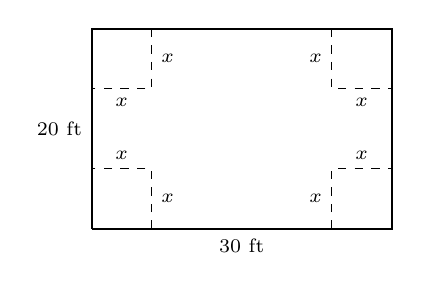
\begin{tikzpicture}
\draw [thick](0,0) -- (1.5in,0) -- (1.5in,1in) -- (0,1in) -- (0,0);
\draw [dashed](0.3in,0) -- (0.3in,0.3in) -- (0,0.3in);
\draw [dashed](1.2in,0) -- (1.2in,0.3in) -- (1.5in,0.3in);
\draw [dashed](1.2in,1in) -- (1.2in,0.7in) -- (1.5in,0.7in);
\draw [dashed](0.3in,1in) -- (0.3in,0.7in) -- (0,0.7in);
\draw [below] (.75in,0) node {\scriptsize $30$ ft};
\draw [left] (0,0.5in) node {\scriptsize $20$ ft};
\draw [below] (.15in,0.7in) node {\scriptsize $x$};
\draw [below] (1.35in,0.7in) node {\scriptsize $x$};
\draw [above] (.15in,0.3in) node {\scriptsize $x$};
\draw [above] (1.35in,0.3in) node {\scriptsize $x$};
\draw [right] (.3in,0.15in) node {\scriptsize $x$};
\draw [right] (.3in,0.85in) node {\scriptsize $x$};
\draw [left] (1.2in,0.15in) node {\scriptsize $x$};
\draw [left] (1.2in,0.85in) node {\scriptsize $x$};
\end{tikzpicture}
\end{minipage}
}
{$\ds x=\frac{25-5\sqrt{7}}{3}\approx 3.92$ in
}

